%%%%%%%%%%%%%%%%%%%%%%%%%%%%%%%%%%%%%%%%%%%%%%%%%%%%%%%%%%%

\section{Apresentação dos dados}

\textbf{Mostrar como são os dados}

% TODO: \usepackage{graphicx} required
\begin{figure}[h!]
	\centering
	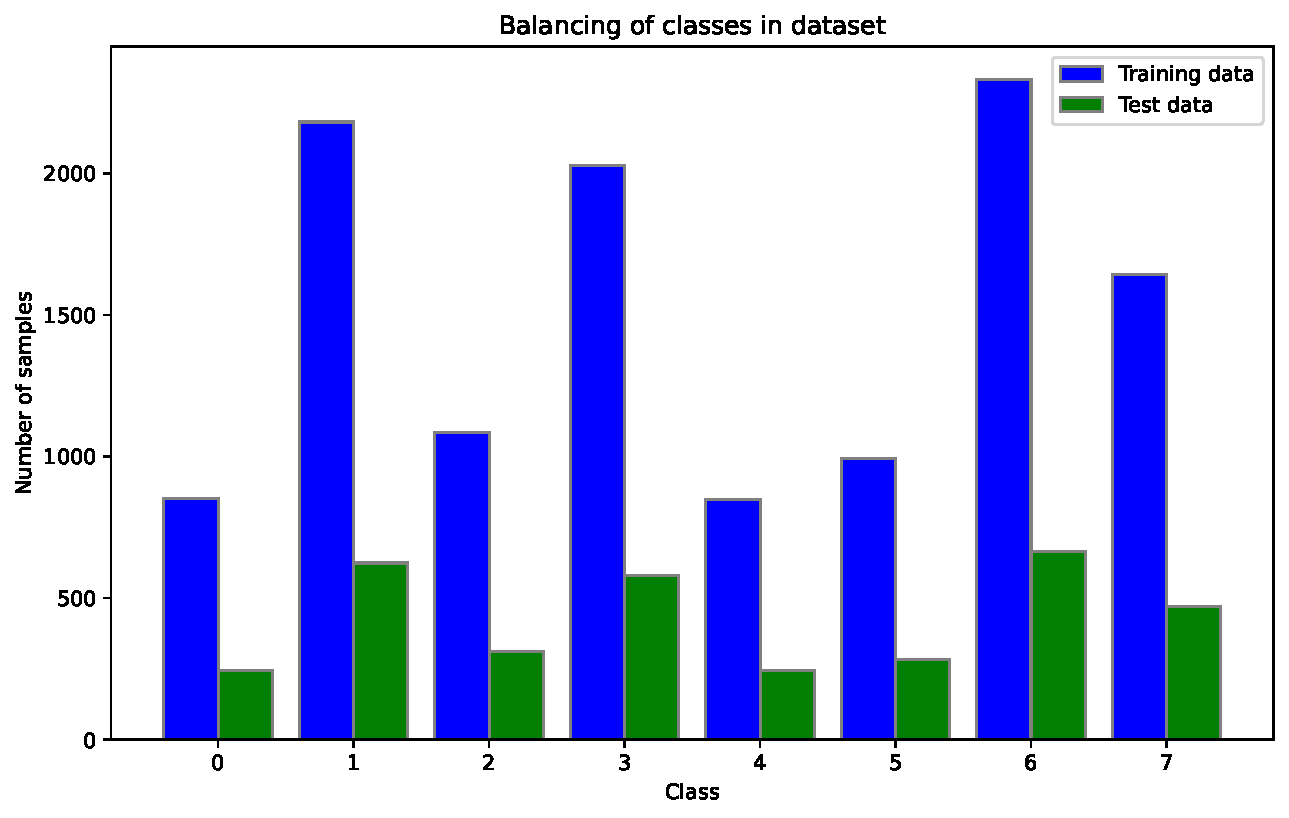
\includegraphics[width=0.75\linewidth]{../../plot/Balancing_of_classes}
	\caption{Balanço das classes nos \textit{datasets} de treinamento e teste.}
	\label{fig:balancingofclasses}
\end{figure}

% TODO: \usepackage{graphicx} required
\begin{figure}[h!]
\centering
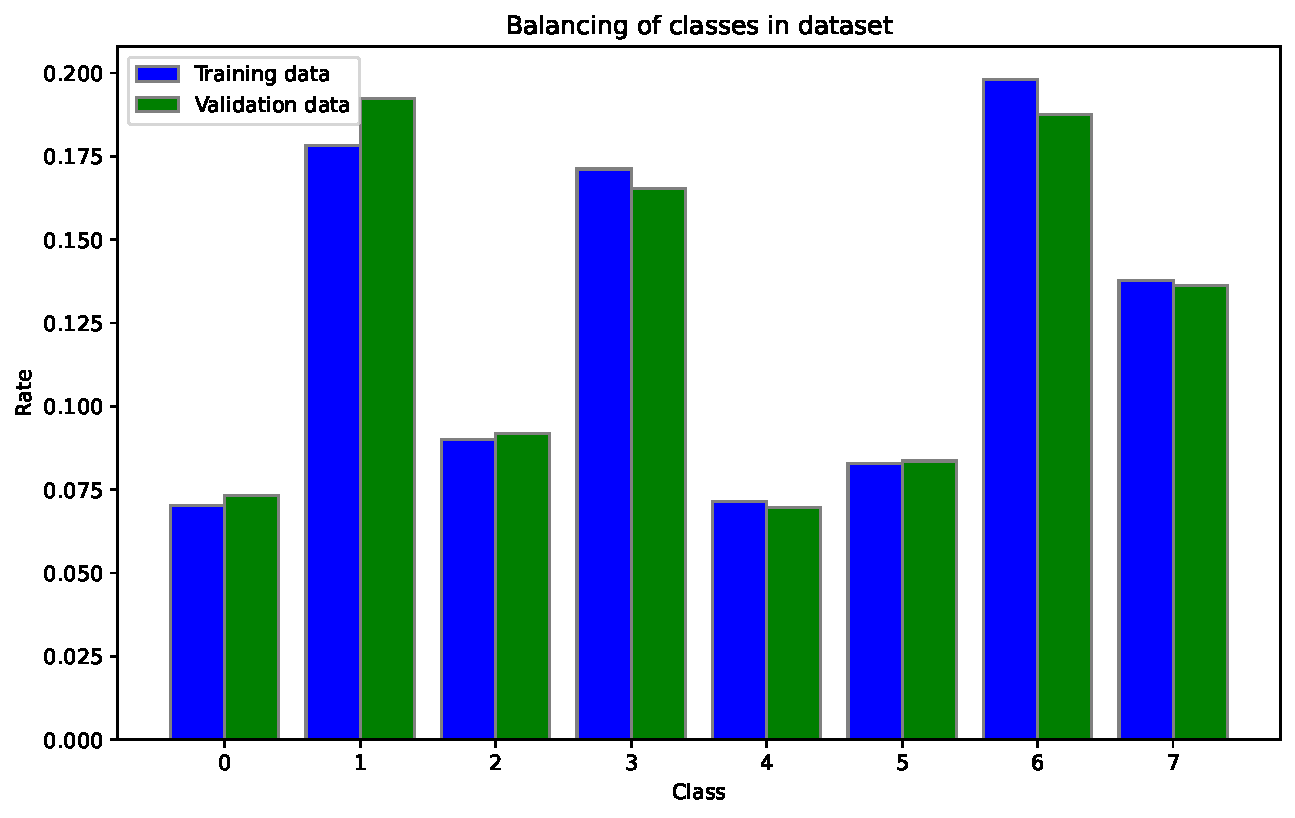
\includegraphics[width=0.75\linewidth]{../../plot/Balancing_of_classes_holdout}
\caption{Balanço das classes nos conjuntos de dados de treinamento e validação cruzada do tipo \textit{holdout}.}
\label{fig:balancingofclasses_holdout}
\end{figure}


\section{MLP}

\subsection{Busca do melhor modelo}


\subsection{Análise do melhor modelo}


\subsubsection{Matriz de confusão}


\subsubsection{Análise dos erros}

